\chapter{Motivation\label{cha:motivation}}
Current contracts between academic publishers and research libraries are based on subscription models, granting patrons of a library almost unlimited access the digital publications of a single publisher. Unfortunately, pricing models often do not correspond to the usage of the publishers content. 
\\
\\
In this paper, we present LibChain, a decentral, verifiable and anonymous access management based on blockchain technology. LibChain envisions a novel procedure to access digital media from different publishers through a library.  With the LibChain service, the library stores every request of a digital publication directly in the blockchain, making it an anonymous but verifiable source for publishers to provide access to the user. The decentral blockchain architecture enables new access models for digital media and allows fairer and more accurate pricing models based on the usage.
\\
\\
LibChain unleashes the full potential if multiple libraries cooperate to create trustworthy usage metrics or share the access to digital publications. As a design principle of the underlying blockchain technology, no mutual trust is required to generate verifiable transactions. 
\\
\\
We explicitly promote open access publications in our system design by providing verifiable usage metrics among distributed libraries and enable anonymous compensations and donations. In addition to a fully described programming interface for established publishers, we provide a standalone toolkit for conferences and smaller research institutes. Hence, small groups of authors can easily contribute to the LibChain universe and act as their own open access publisher.
\\
\\
The implementation of our research prototype is based on the open source blockchain framework ethereum. The key advantages of LibChain are: First, it provides a distributed, failure tolerant mechanism for free, open and anonymous access to content that can be used out-of-the-box by anyone. Second, it is compatible to conventional business models, where publishers sell their content for a predefined price. This compatibility is aimed to accelerate the adoption of LibChain by maximising network-external value by integrating the open access and payed publication segments. Third, LibChain provides a reliable way to measure the impact of content and realise payments, since due to its blockchain core, all interactions with LibChain can be verified and trusted. Fourth, LibChain balances the access to information relevant to content providers and the privacy needs of users. Given these advantages, LibChain has the potential to accelerate the shift to an open access publication model that provides a robust, distributed content exchange mechanism and substantially higher utility than conventional models to all involved parties.

\imp{muss noch angepasst werden !!!}
\chapter{Blockchain Technology\label{cha:chapter1}}

A blockchain is a distibuted database that stores informations on linked blocks. To ensure the integrity of the information, every block includes a hash value of its previous block and a Merkel Root of all transactions in the block. Modifications on a confirmed block would lead to a different hashvalue. Therefore, manipulating informations on a blockchain is very hard and provides a high level of reliability.
Informations are stored on the blockchain through transactions. The validity of transactions are verified by miners and are bundeled up to blocks. Miners have to provide a Proof-of-Work in order for their verification of a new block to be accepted by the rest of the network. The chain of blocks with the most amount of Proof-of-Work is where new blocks should be added to. 

\vspace{0.3cm}
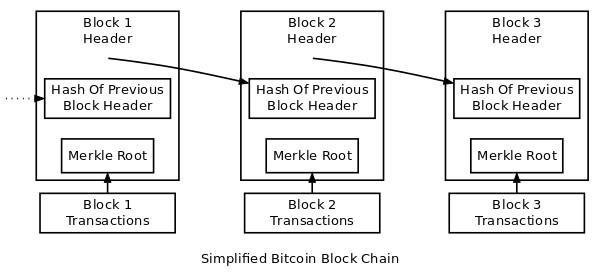
\includegraphics[width=\textwidth]{blockchain.jpg}\footnote{(http://bitcoin.stackexchange.com/questions/35448/is-it-chain-of-headers-rather-than-a-chain-of-blocks)}

Blockchains became mainly known in a financial context. The first implementation of a blockchain was used by Bitcoin, a virtual distributed crypto currency.
But in the meantime, blockchain technology has also become popular in other domains i.e. Voting-Systems \ref{yermack2017corporate} or for digital identity management \ref{isaen}. Applications that needs a high level of integrity and reliablilty could benefit from blockchains.

\imp{not finished, refs dont work?}


%\begin{itemize}
%\item What is blockchain technology?
%\item Advantages and how to use these to serve new business models?
%\item what are the well known implementations of a blockchain? (Bitcoin, Ethereum)
%\end{itemize}

\section{Ethereum}
Ethereum is a public blockchain we used for LibChain, that allows us to implement decentralized applications by means of "Smart Contracts". A smart contract is exectuable code that is stored on the blockchain. It is accessible through a unique address and triggered through transaction calls.
To execute a transaction so called gas is consumed. Gas is the fuel that is being used to pay the execution fee of the transaction\footnote{\url{http://www.reddit.com/r/ethereum/comments/2udvau/what_is_the_difference_between_gas_and_ether/}}.

The programming language to implement contracts is called \textit{Solidity}. It's a high-level turing complete programming language whose syntax is similar to JavaScript. Contracts are collections of functions and variables:

\begin{lstlisting}
contract SimpleStorage {
    uint storedData;

    function set(uint x) {
        storedData = x;
    }

    function get() constant returns (uint) {
        return storedData;
    }
}
\end{lstlisting}\footnote{\url{http://solidity.readthedocs.io/en/develop/introduction-to-smart-contracts.html}}


Mining a block on the Ethereum blockchain involves verification that exactly the deployed code was executed without tempering or inconsistencies between versions. Due to this transparency, it's easy to implement applications where normally a high level of trust between participants is needed.